\subsection{Cuándo llega la carga a los 900 grados}
\label{sec:calentamiento}

Casi todo lo que se observa entre los \num{30} y los \SI{150}{\second} está
gobernado por el reloj térmico y no por la química: la mufla está a
\SI{900}{\celsius} desde el principio, pero el aglomerado no. Conviene fijar ese
reloj en números antes de discutir ninguna reacción.

\begin{figure}[H]
\centering
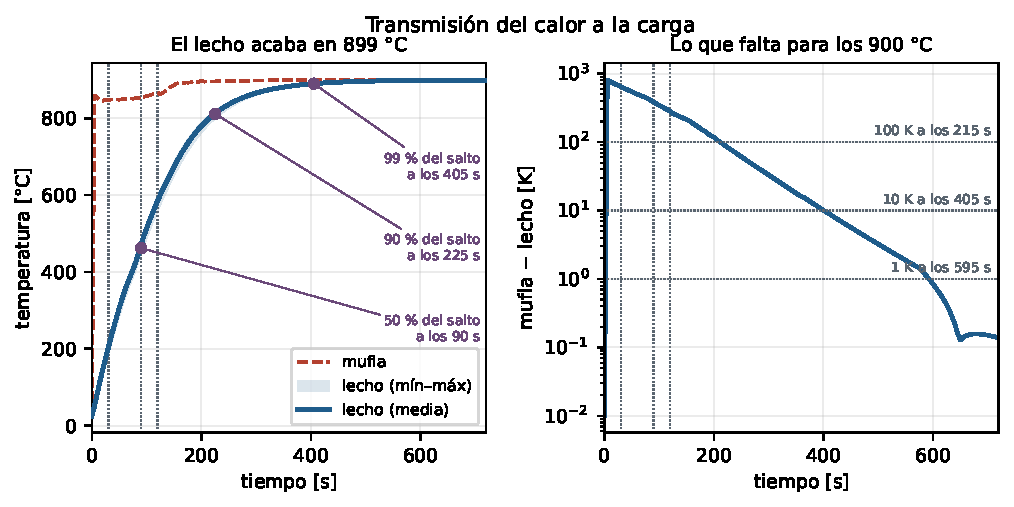
\includegraphics[width=\textwidth]{fig_fen_calentamiento}
\caption{Transmisión del calor a la carga. A la izquierda, la temperatura media
del lecho con su banda mínimo--máximo y los tres hitos del salto térmico. A la
derecha, lo que le falta al lecho para alcanzar a la mufla, en escala
logarítmica: si hubiese una sola constante de tiempo sería una recta, y no lo
es, porque mientras dura la devolatilización el gas que sale se lleva calor y
la pirólisis lo absorbe.}
\label{fig:calentamiento}
\end{figure}

El lecho recorre la mitad del salto térmico a los \datCalorMitad\
\si{\second}, el \SI{90}{\percent} a los \datCalorNoventa\ \si{\second} y el
\SI{99}{\percent} a los \datCalorNoventaNueve\ \si{\second}. Se pone a menos de
\SI{100}{\kelvin} de la mufla a los \datFaltaCien\ \si{\second}, a menos de
\SI{10}{\kelvin} a los \datFaltaDiez\ y a menos de \SI{1}{\kelvin} a los
\datFaltaUno. Acaba el ensayo en \datTLechoFinal\ \si{\celsius}: nunca llega a
tocar los \SI{900}{\celsius} exactos, se les acerca asintóticamente.

Dos cosas de esta figura importan más allá de lo descriptivo.

La primera es que \textbf{el hito de los \SI{90}{\second} cae sobre el cruce de
la ventana termoplástica, no cerca}: en ese instante el lecho pasa por
\datTLechoNoventa\ \si{\celsius}, dentro de \SIrange{350}{500}{\celsius}. Que
el laboratorio viera hinchamiento justo ahí no es una coincidencia que el
modelo tenga que explicar después: es la predicción del reloj térmico, hecha
sin ninguna constante química.

La segunda es un corolario que se usa en \S\ref{sec:reduccion-incompleta}:
\textbf{la ventana en la que hay reductor y temperatura a la vez es estrecha}.
La devolatilización se agota hacia los \SI{150}{\second}, y el lecho no alcanza
el \SI{99}{\percent} del salto hasta los \datCalorNoventaNueve\ \si{\second}.
Cuando el sólido llega por fin a la temperatura a la que la cinética de
reducción sería rápida, el gas reductor ya se ha ido. Las dos condiciones
apenas se solapan, y ese desencuentro ---no la falta de carbono--- es parte de
por qué la conversión se queda donde se queda.
